\documentclass{article}
\usepackage[utf8]{inputenc}
\usepackage[italian]{babel}
\usepackage{amsmath}
\usepackage{siunitx}
\usepackage{tabularray}
\usepackage{graphicx}
\title{
    Laboratorio di Fisica 1\\
    R2: Misura costante elastica di una molla
}
\author{Gruppo 17: Bergamaschi Riccardo, Graiani Elia, Moglia Simone}
\date{04/10/2023 – 11/10/2023}
\makeindex
\begin{document}

\maketitle

\begin{abstract}
    Il gruppo di lavoro ha misurato la costante elastica di una molla con due metodi distinti.
\end{abstract}

\section{Materiali e strumenti di misura utilizzati}
\begin{center}
    \begin{tblr}{ |Q[l,m]|Q[c,m]|Q[c,m]|Q[c,m]| }
        \hline
        \textbf{Strumento di misura} & \textbf{\:\:\:\:Soglia\:\:\:\:} & \textbf{Portata} & \textbf{Sensibilità} \\
        \hline
        {Fototraguardo con \\ contatore di impulsi} & \qty{1}{\micro s} & \qty{99999999}{\micro s} & \qty{1}{\micro s} \\
        \hline[dashed]
        Righello & \qty{0.1}{cm} & \qty{60.0}{cm} & \qty{0.1}{cm} \\
        \hline[dashed]
        Bilancia di precisione & \qty{0.01}{g} & \qty{6200.00}{g} & \qty{0.01}{g} \\
        \hline
        \hline
        \textbf{Altro} & \SetCell[c=3]{l} \textbf{Descrizione/Note} \\
        \hline
        Molla e gancio & \SetCell[c=3]{l} {
            Un estremo della molla è vincolato ad un \\
            supporto fisso, mentre all'altro è appeso \\
            un gancio per agevolare il caricamento dei \\
            campioni
        } \\
        \hline[dashed]
        {Tre campioni solidi \\ (con masse distinte)} & \SetCell[c=3]{l} {
            Indicheremo con $A,B,C$ i tre campioni \\
            e con $A+B$, $A+C$, $B+C$ e $A+B+C$ \\
            le loro combinazioni. Tutti questi saranno \\
            qui chiamati “gravi”.
        } \\
        \hline[dashed]
        Specchio & \SetCell[c=3]{l} {
            Posizionato verticalmente dietro al righello, \\
            permette di ridurre eventuali errori di let- \\
            tura dovuti all'effetto di parallasse
        } \\
        \hline[dashed]
        Livella & \SetCell[c=3]{l} {
            Utile per assicurarsi che il fototraguardo \\
            sia orizzontale
        } \\
        \hline
    \end{tblr}
\end{center}

% *questi strumenti di misura, seppur disponibili, non sono stati
% utilizzati a causa della loro elevata sensiblità.

\section{Esperienza e procedimento di misura}
\subsection{Misurazione della costante elastica nel caso statico}
\begin{enumerate}
    \item Fissiamo il righello parallelo a $\vec{g}$ e solidale
          all’estremo fisso della molla.
          Individuiamo allora un punto $P$ del sistema, solidale all’estremo
          libero della molla, che terremo come riferimento per misurare
          (indirettamente) gli allungamenti.
    \item Misuriamo allora la posizione $x_0$ di $P$
          (rispetto allo 0 del righello) senza caricare
          alcuna massa sui ganci: possiamo considerare questa la
          lunghezza a riposo della molla, in quanto il contributo
          della massa della molla e del gancio, nel caso statico, si annulla.
    \item Per ogni grave\footnotemark[1] $i$:
    \begin{enumerate}
        \item Ne misuriamo la massa $m_i$ con la bilancia di precisione
              (nel caso di combinazioni di più campioni, ne misuriamo
              direttamente la massa complessiva);
        \item Appeso il grave alla molla, ne misuriamo indirettamente l'allungamento
        $\left(\Delta x\right)_i$, sottraendo $x_0$ alla misura $x_i$
        della sua posizione (e allora $\delta (\Delta x)_i = \delta x_0 + \delta x_i$).
        Per ridurre ulteriormente la probabilità di commettere errori di parallasse,
        ripetiamo il procedimento tre volte, tenendo solamente la misura più vicina alla media.
    \end{enumerate}
\end{enumerate}


Di seguito sono riportate le misure così ottenute:
\[x_0 = \left(3.3\pm 0.1\right)\unit{cm}\]

\begin{center}\begin{tblr}{ |c|c|c|c| }
    \hline
        {\textbf{Grave} \\ $i$} &
        {\textbf{Massa} \\ $m_i$ (\unit{g})} &
        {\textbf{Posizione} \\ $x_i$ (\unit{cm})} &
        {\textbf{Allungamento} \\ $\left(\Delta x\right)_i$ (\unit{cm})} \\
    \hline
    $A$     & $  407,73\:\pm\:0.01$ & $ 7,9\:\pm\:0.1$ & $ 4,6\:\pm\:0.2$ \\
    $B$     & $  542,47\:\pm\:0.01$ & $ 9,6\:\pm\:0.1$ & $ 6,3\:\pm\:0.2$ \\
    $C$     & $  667,82\:\pm\:0.01$ & $11,3\:\pm\:0.1$ & $ 8,0\:\pm\:0.2$ \\
    $A+B$   & $  950,22\:\pm\:0.01$ & $14,4\:\pm\:0.1$ & $11,1\:\pm\:0.2$ \\
    $A+C$   & $ 1085,56\:\pm\:0.01$ & $15,9\:\pm\:0.1$ & $12,6\:\pm\:0.2$ \\
    $B+C$   & $ 1220,28\:\pm\:0.01$ & $17,5\:\pm\:0.1$ & $14,2\:\pm\:0.2$ \\
    $A+B+C$ & $ 1628,02\:\pm\:0.01$ & $22,2\:\pm\:0.1$ & $18,9\:\pm\:0.2$ \\
    \hline
\end{tblr}\end{center}

Per determinare la costante elastica $k$ della molla, abbiamo effettuato
una regressione lineare (non pesata) dei dati così ottenuti, facendo
riferimento alla seguente formula (che segue direttamente dalla legge
di Hooke, ponendo $F_\text{elastica}$ = $F_\text{peso}$):
\[\Delta x = \frac{g}{k} m\]
Detto $b=b_\text{best}\pm\delta b$ il coefficiente angolare della retta di regressione, vale allora:
\[
    k = \frac{g_\text{best}}{b_\text{best}}\qquad\wedge\qquad
    \frac{\delta k}{k_\text{best}} = \frac{\delta g}{g_\text{best}} + \frac{\delta b}{b_\text{best}}
\]
Si noti che l'intercetta della retta di regressione dev'essere compatibile con $0$.

\emph{
    \textbf{Osservazione}.
    $g$ non può essere considerata una costante nota con certezza,
    poiché, secondo la legge di gravitazione universale, $g$ dipende
    dalla distanza dal centro di massa della Terra: che $g$ sia costante
    lungo la traiettoria del sistema molla-grave è soltanto
    un'approssimazione. Pertanto, abbiamo considerato
    $g=\left(9.81\pm0.01\right)\unit{m\per s^2}$
}

Ecco la retta di regressione (in rosa è indicata la fascia di confidenza) e i relativi risultati:
\begin{figure}[ht]
    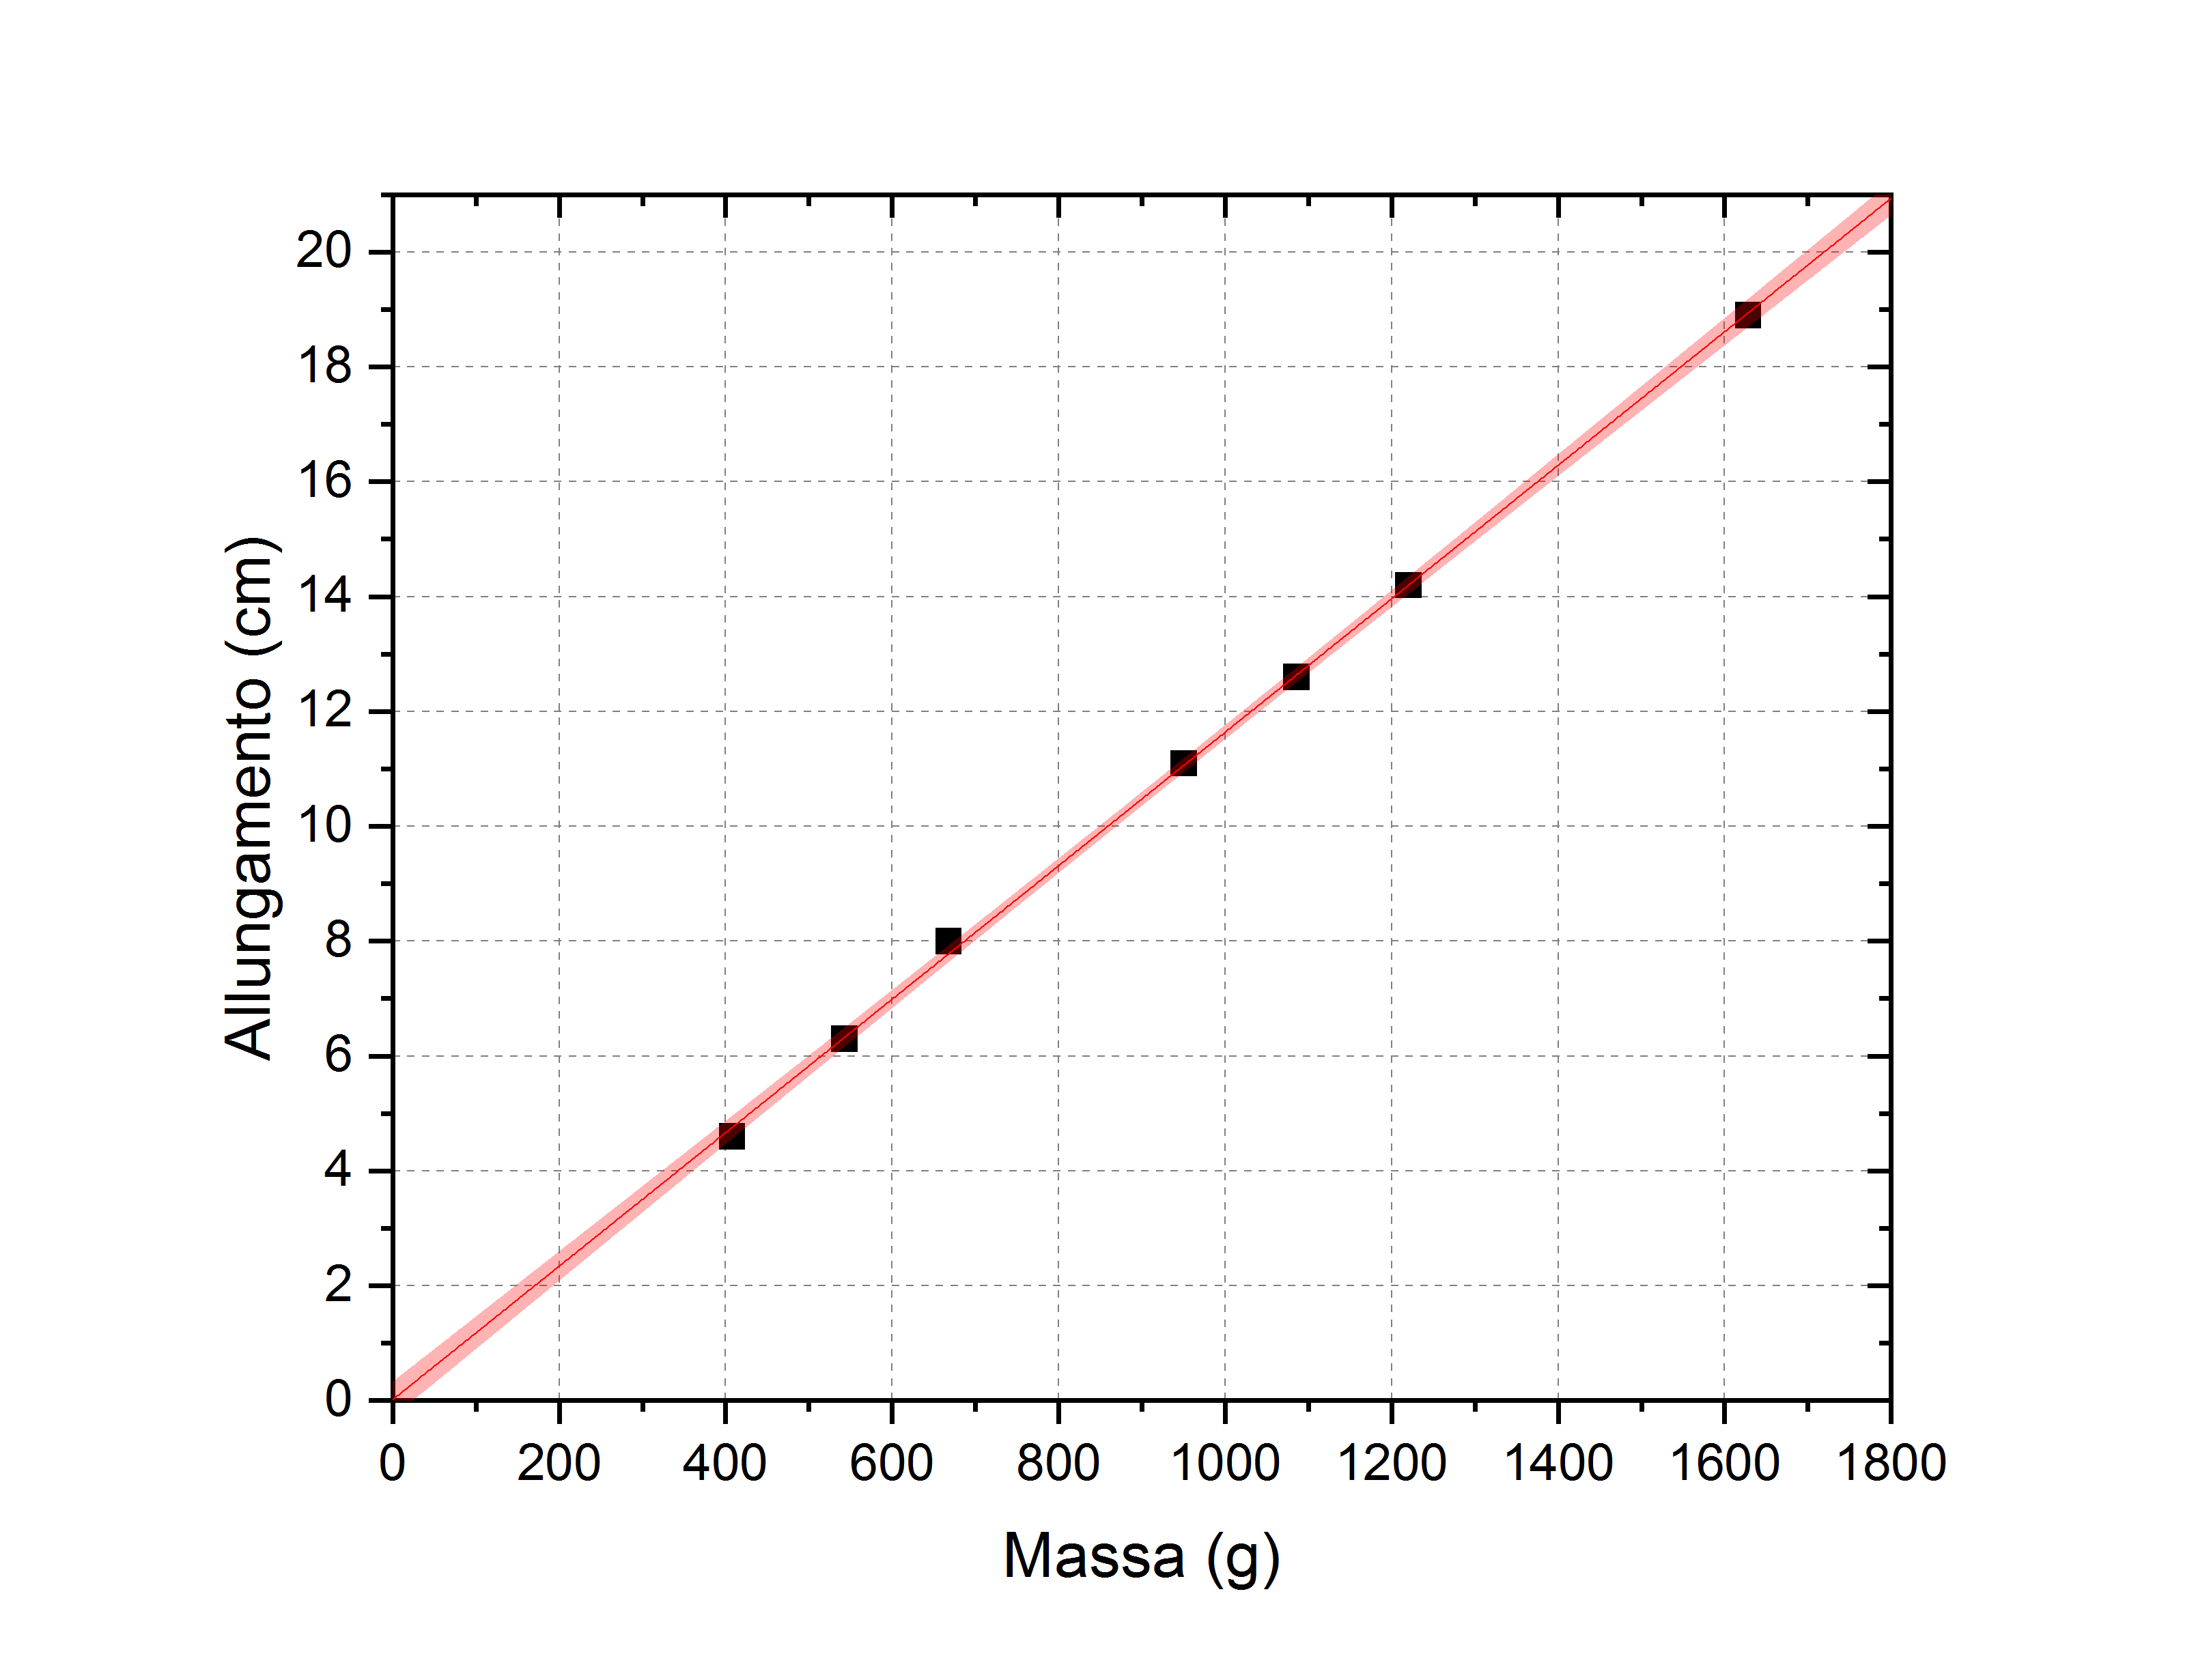
\includegraphics[trim={0 1.8cm 0 0},width=\textwidth]{SaticoReg.jpg}
    \caption{Retta di regressione (in rosso) e la sua regione di incertezza (in rosa).}
\end{figure}
\begin{itemize}
    \item $a = \left(0.02\pm0.12\right)\unit{cm}$ (compatibile con 0)
    \item $
        b = \left(11.62\pm0.12\right)\cdot10^{-3}\unit{cm\per g}
          = \left(11.62\pm0.12\right)\cdot10^{-2}\unit{m\per kg}
    $
    \item $k = \left(84.4\pm0.8\right)\unit{N\per m}$
\end{itemize}

\subsection{Misurazione della costante elastica nel caso dinamico}
\begin{enumerate}
    \item Acceso il contatore di impulsi, lo impostiamo in modo tale che,
          dopo aver avviato l'acquisizione dati, esso misuri venti periodi
          dell'oscillazione.
    \item Per ogni grave $i$ fra i quattro più leggeri\footnotemark[1] ($A, B, C$ e $A+B$):
    \begin{enumerate}
        \item Appeso il campione alla molla, allineiamo i due fototraguardi
              aiutandoci con la livella, in modo tale che possano rilevare
              le oscillazioni nel modo più accurato possibile;
        \item Tiriamo leggermente il campione verso il basso e poi lo rilasciamo,
              in modo che il sistema molla inizi a oscillare con direzione
              il più possibile parallela a $\vec{g}$;
        \item Attesa la stabilizzazione dell’oscillazione, avviamo
              l'acquisizione della misura di 20 periodi $20T_i$.
    \end{enumerate}
    \item Infine, misuriamo con la bilancia, separatamente,
          la massa della molla $m_m$ e la massa del gancio $m_g$.
\end{enumerate}

Infatti, nel caso dinamico, il contributo di queste masse
\emph{non} si annulla; in particolare, la massa del gancio
contribuisce appieno (in quanto è solidale col grave),
mentre la massa della molla contribuisce per circa
$\frac{1}{3}$. La massa effettiva da considerare per ogni grave
sarà allora:
\[\left(\left(m_\text{eff}\right)_i\right)_\text{best} = \left(m_i\right)_\text{best} + \left(m_g\right)_\text{best} + \frac{1}{3}\left(m_m\right)_\text{best}\]
\[\delta \left(m_\text{eff}\right)_i = \delta m_i + \delta m_g + \frac{1}{3}\delta m_m\]

Di seguito sono riportate le distribuzioni dei dati raccolti:

\begin{figure}[ht]
    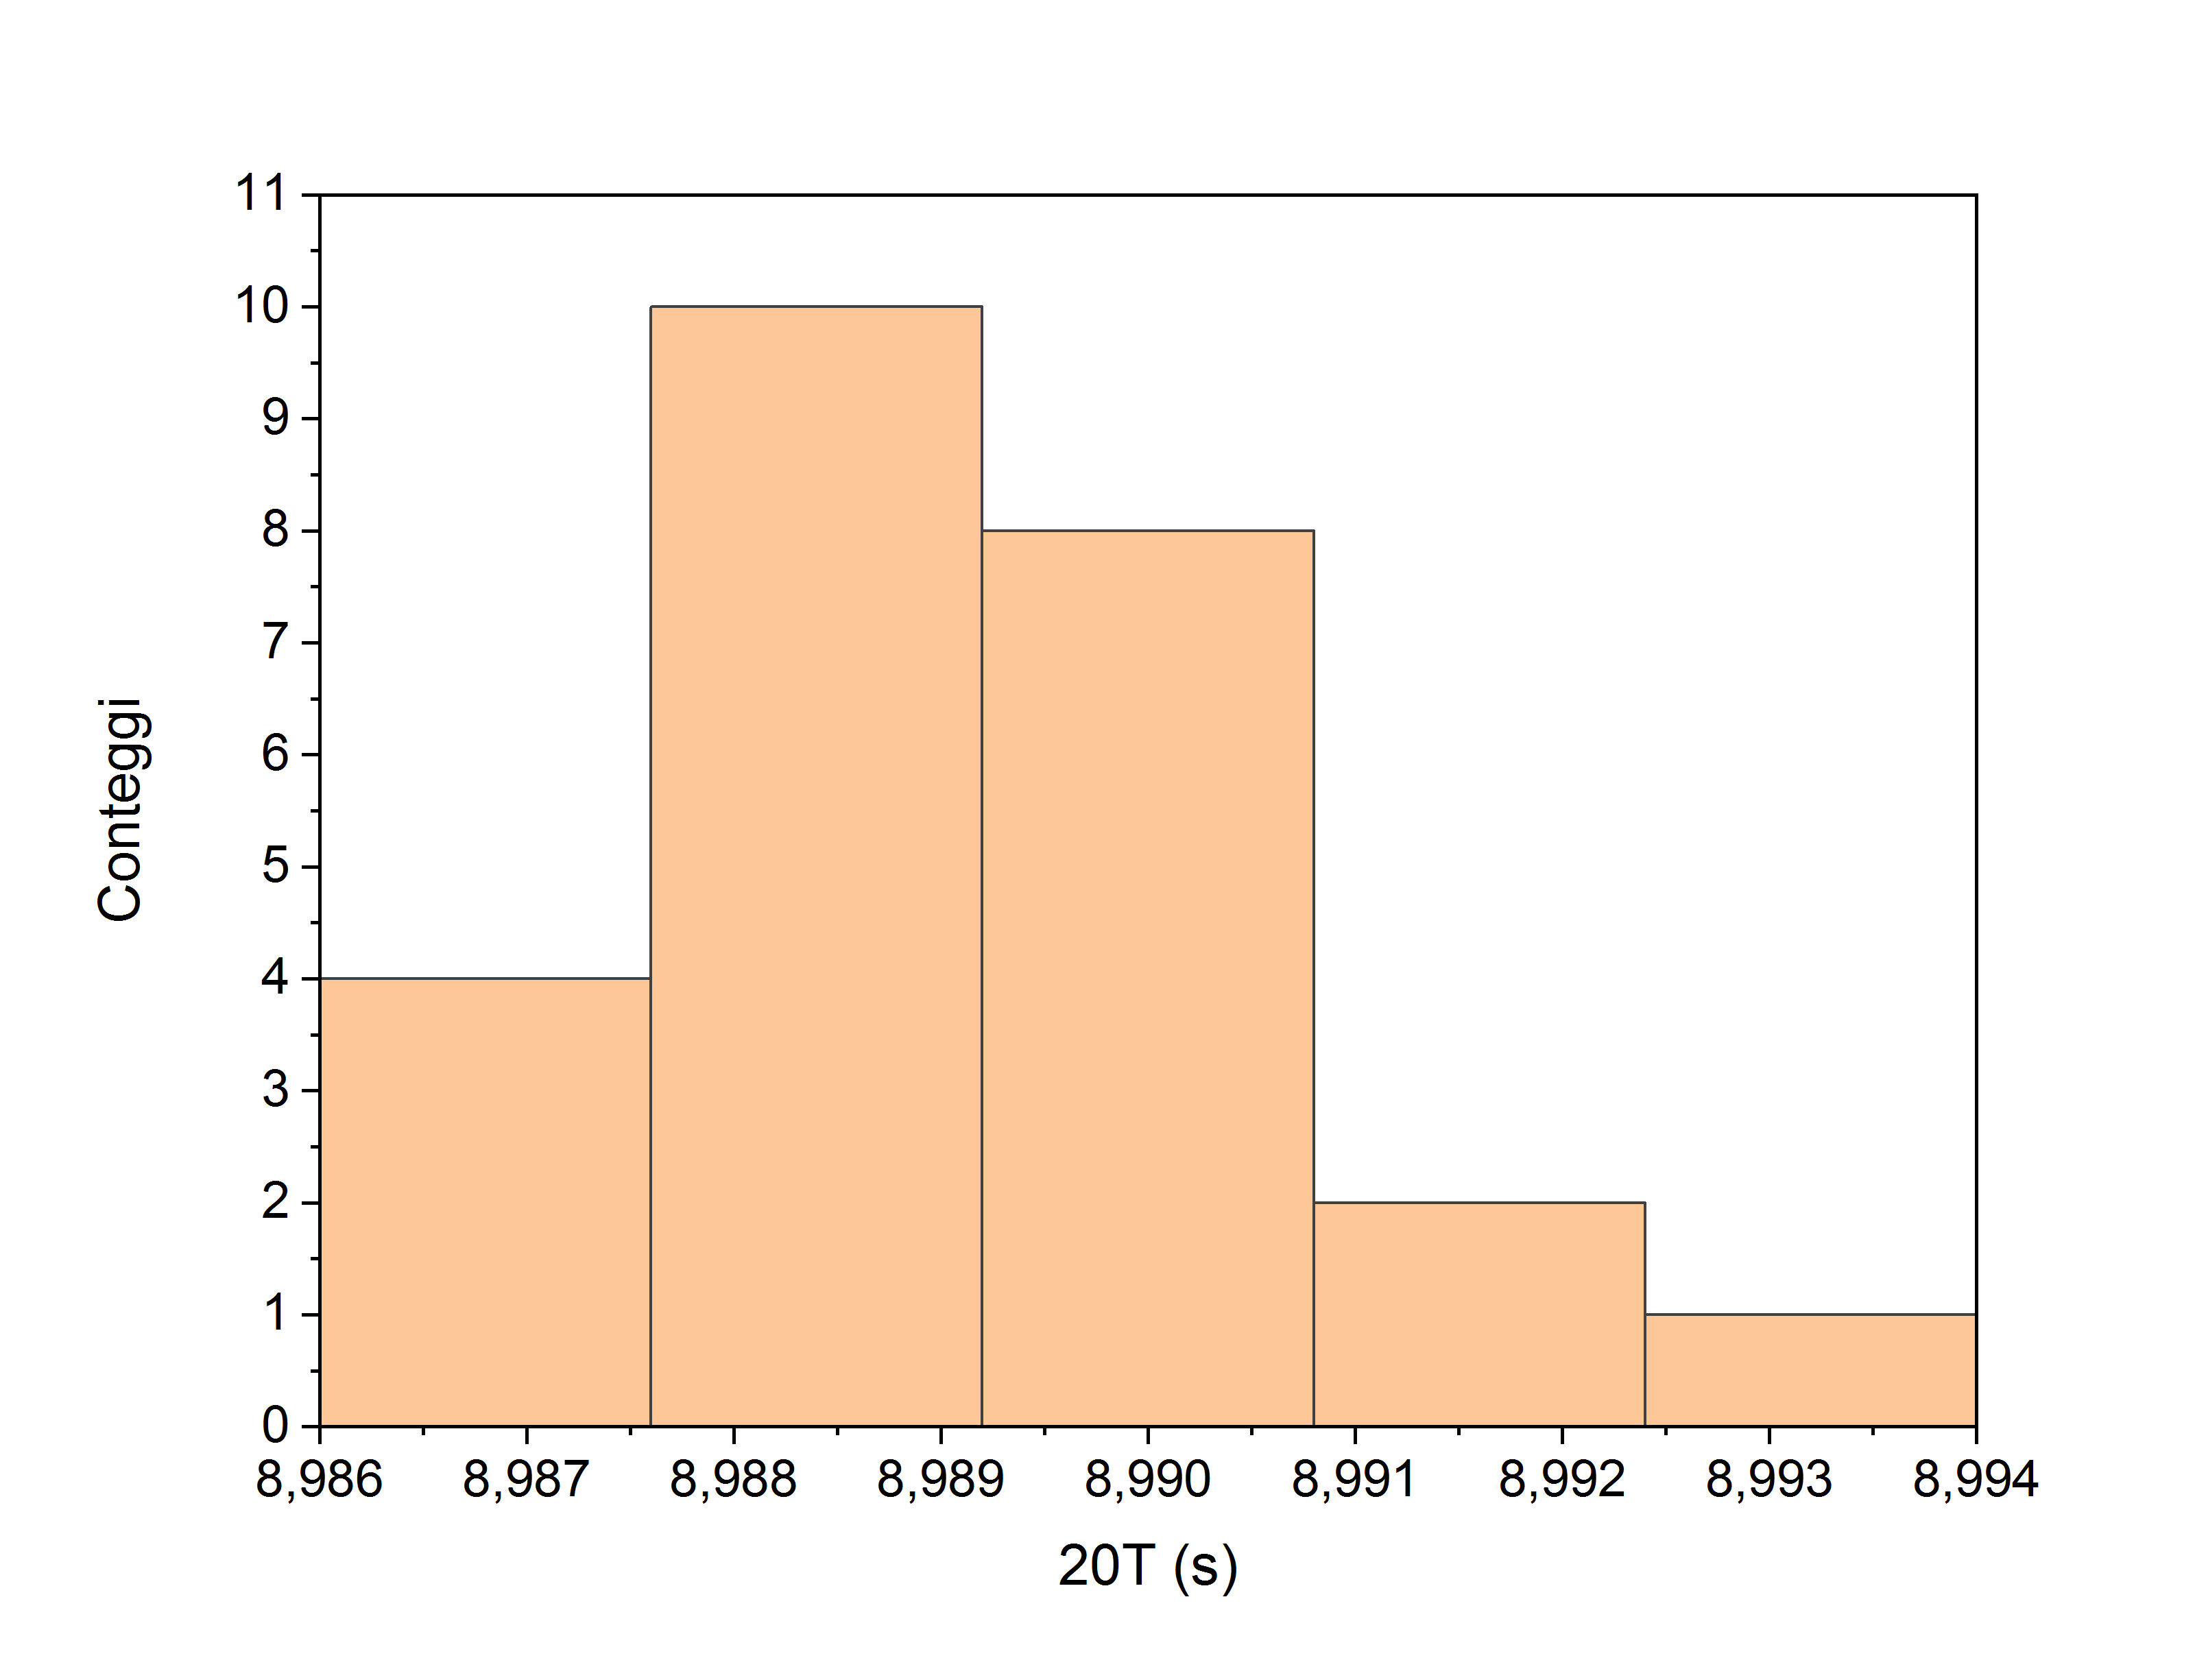
\includegraphics[trim={2cm 1.8cm .7cm 1.5cm},width=.5\textwidth]{Dinamico1.jpg}
    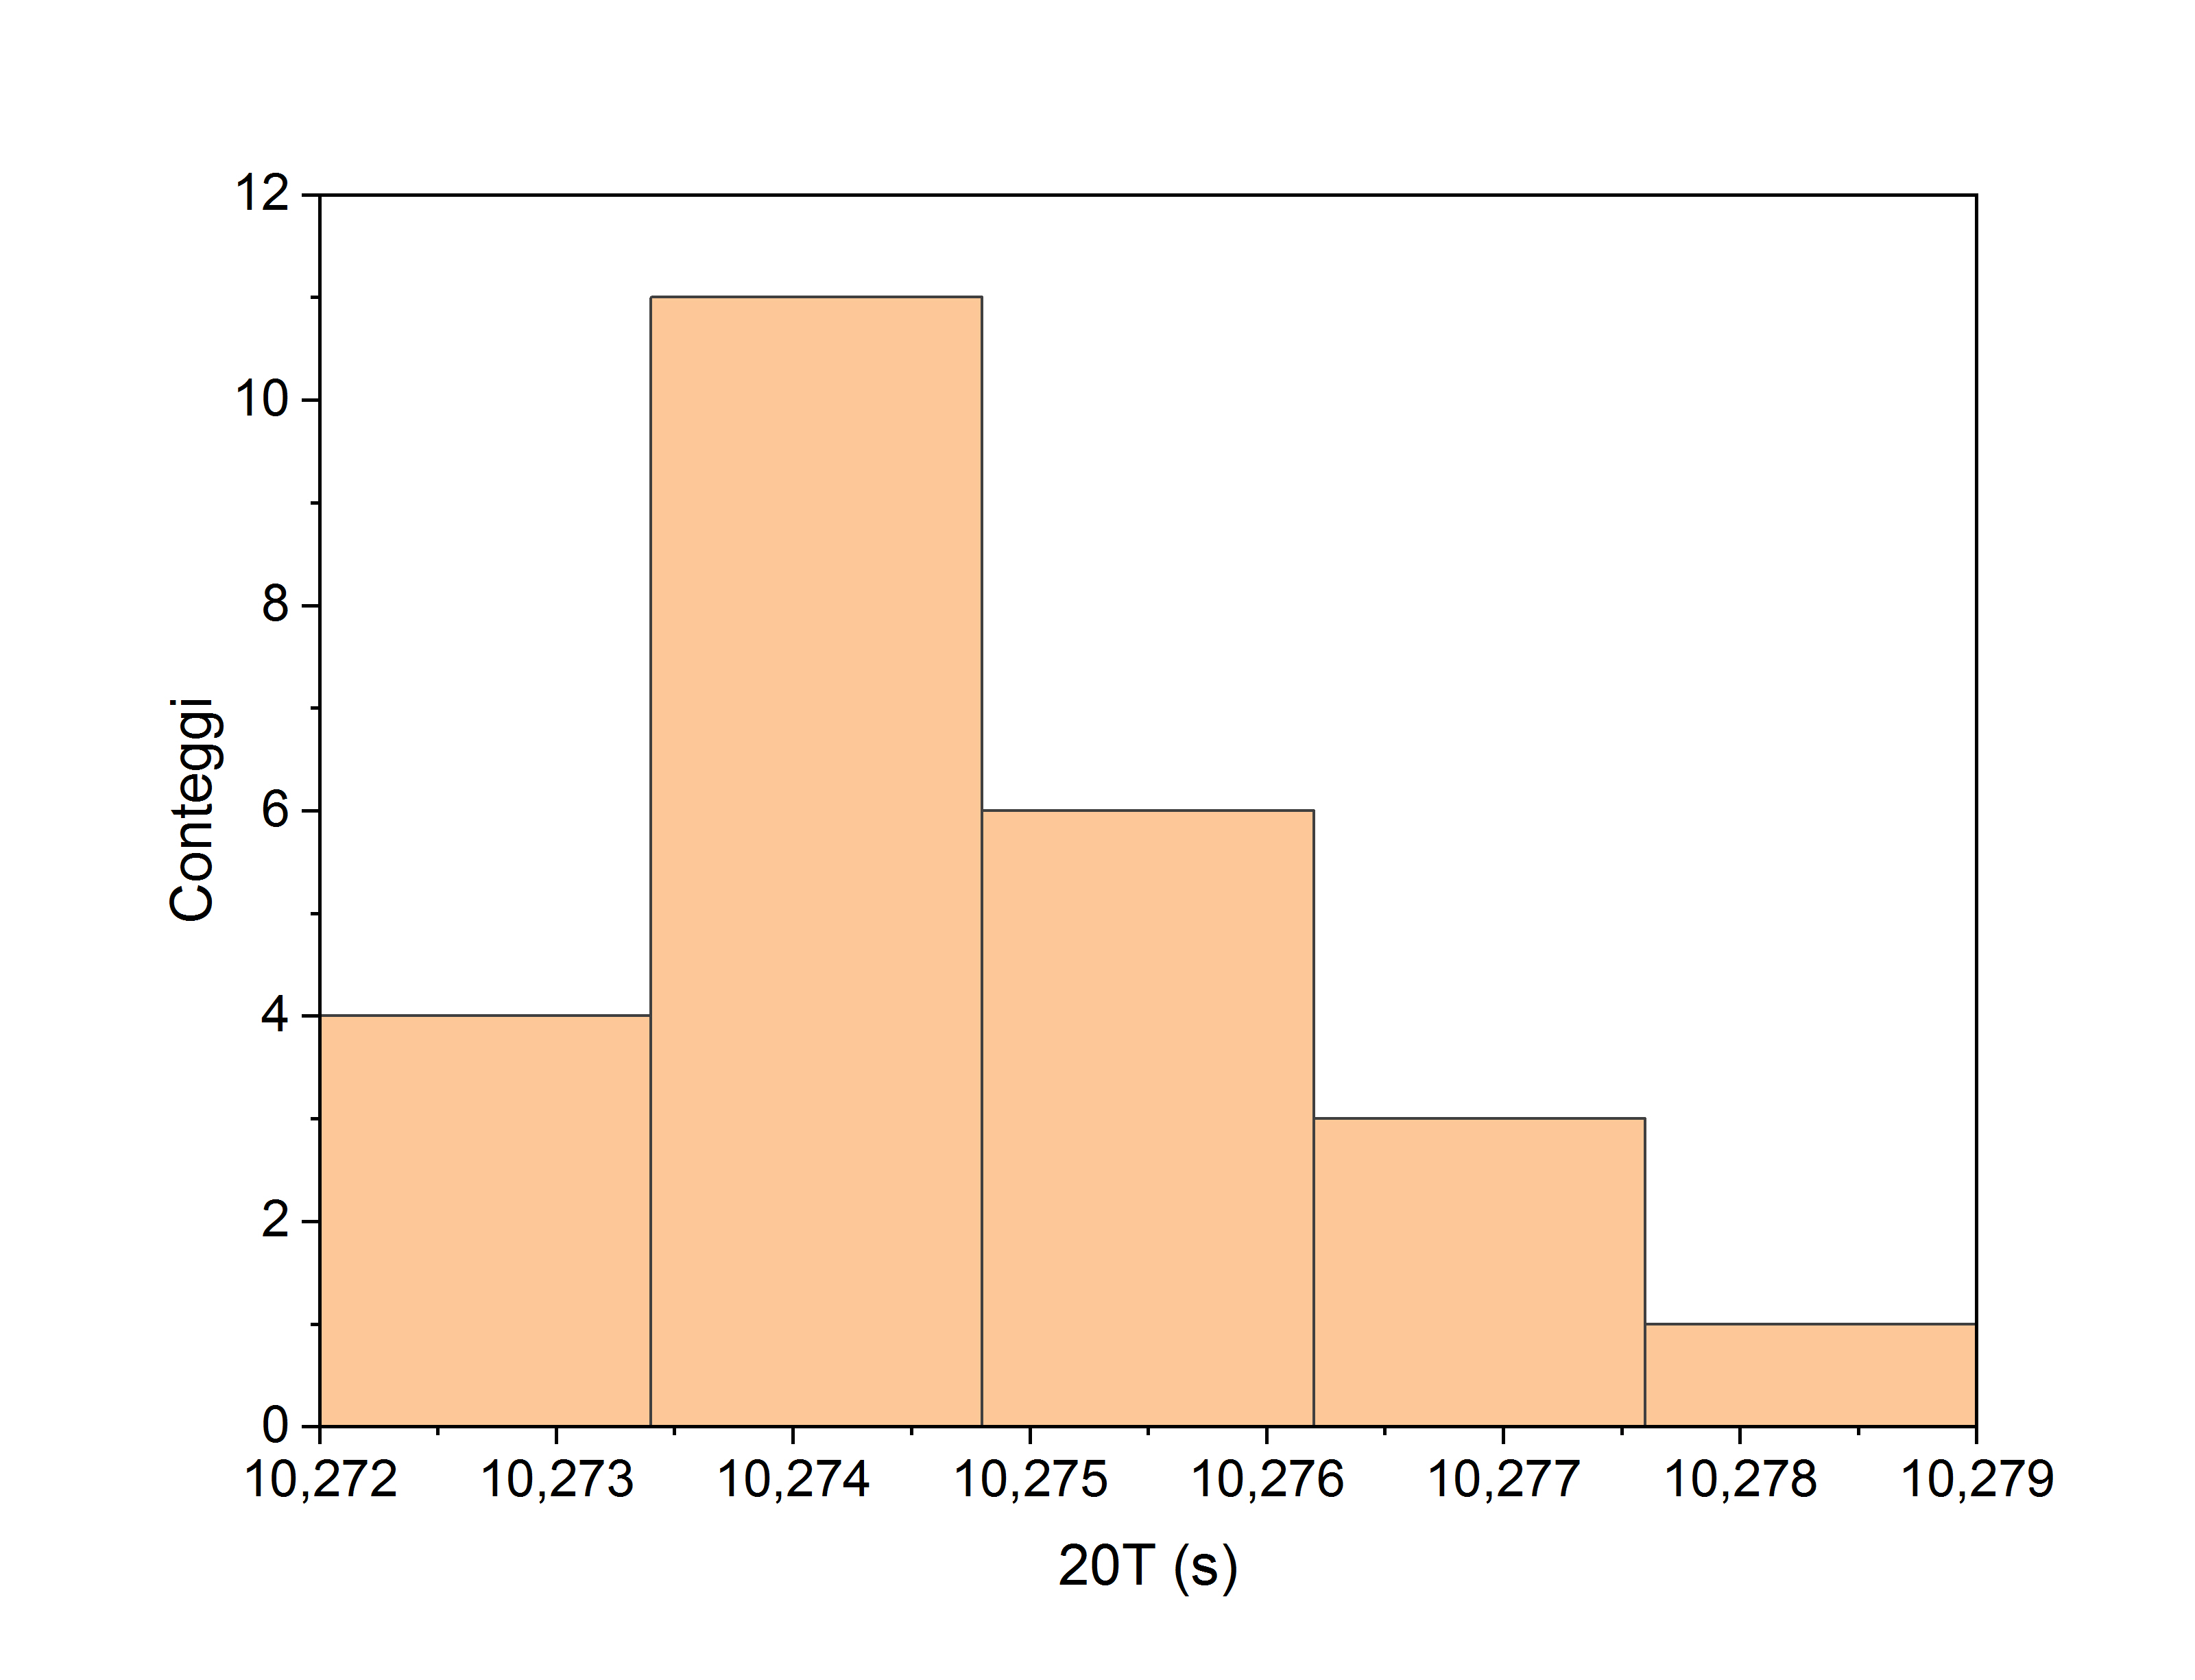
\includegraphics[trim={.7cm 1.8cm 2cm 1.5cm},width=.5\textwidth]{Dinamico2.jpg}
    \caption{Istogrammi dei periodi delle oscillazioni di $A$ e $B$}
\end{figure}\begin{figure}[ht]
    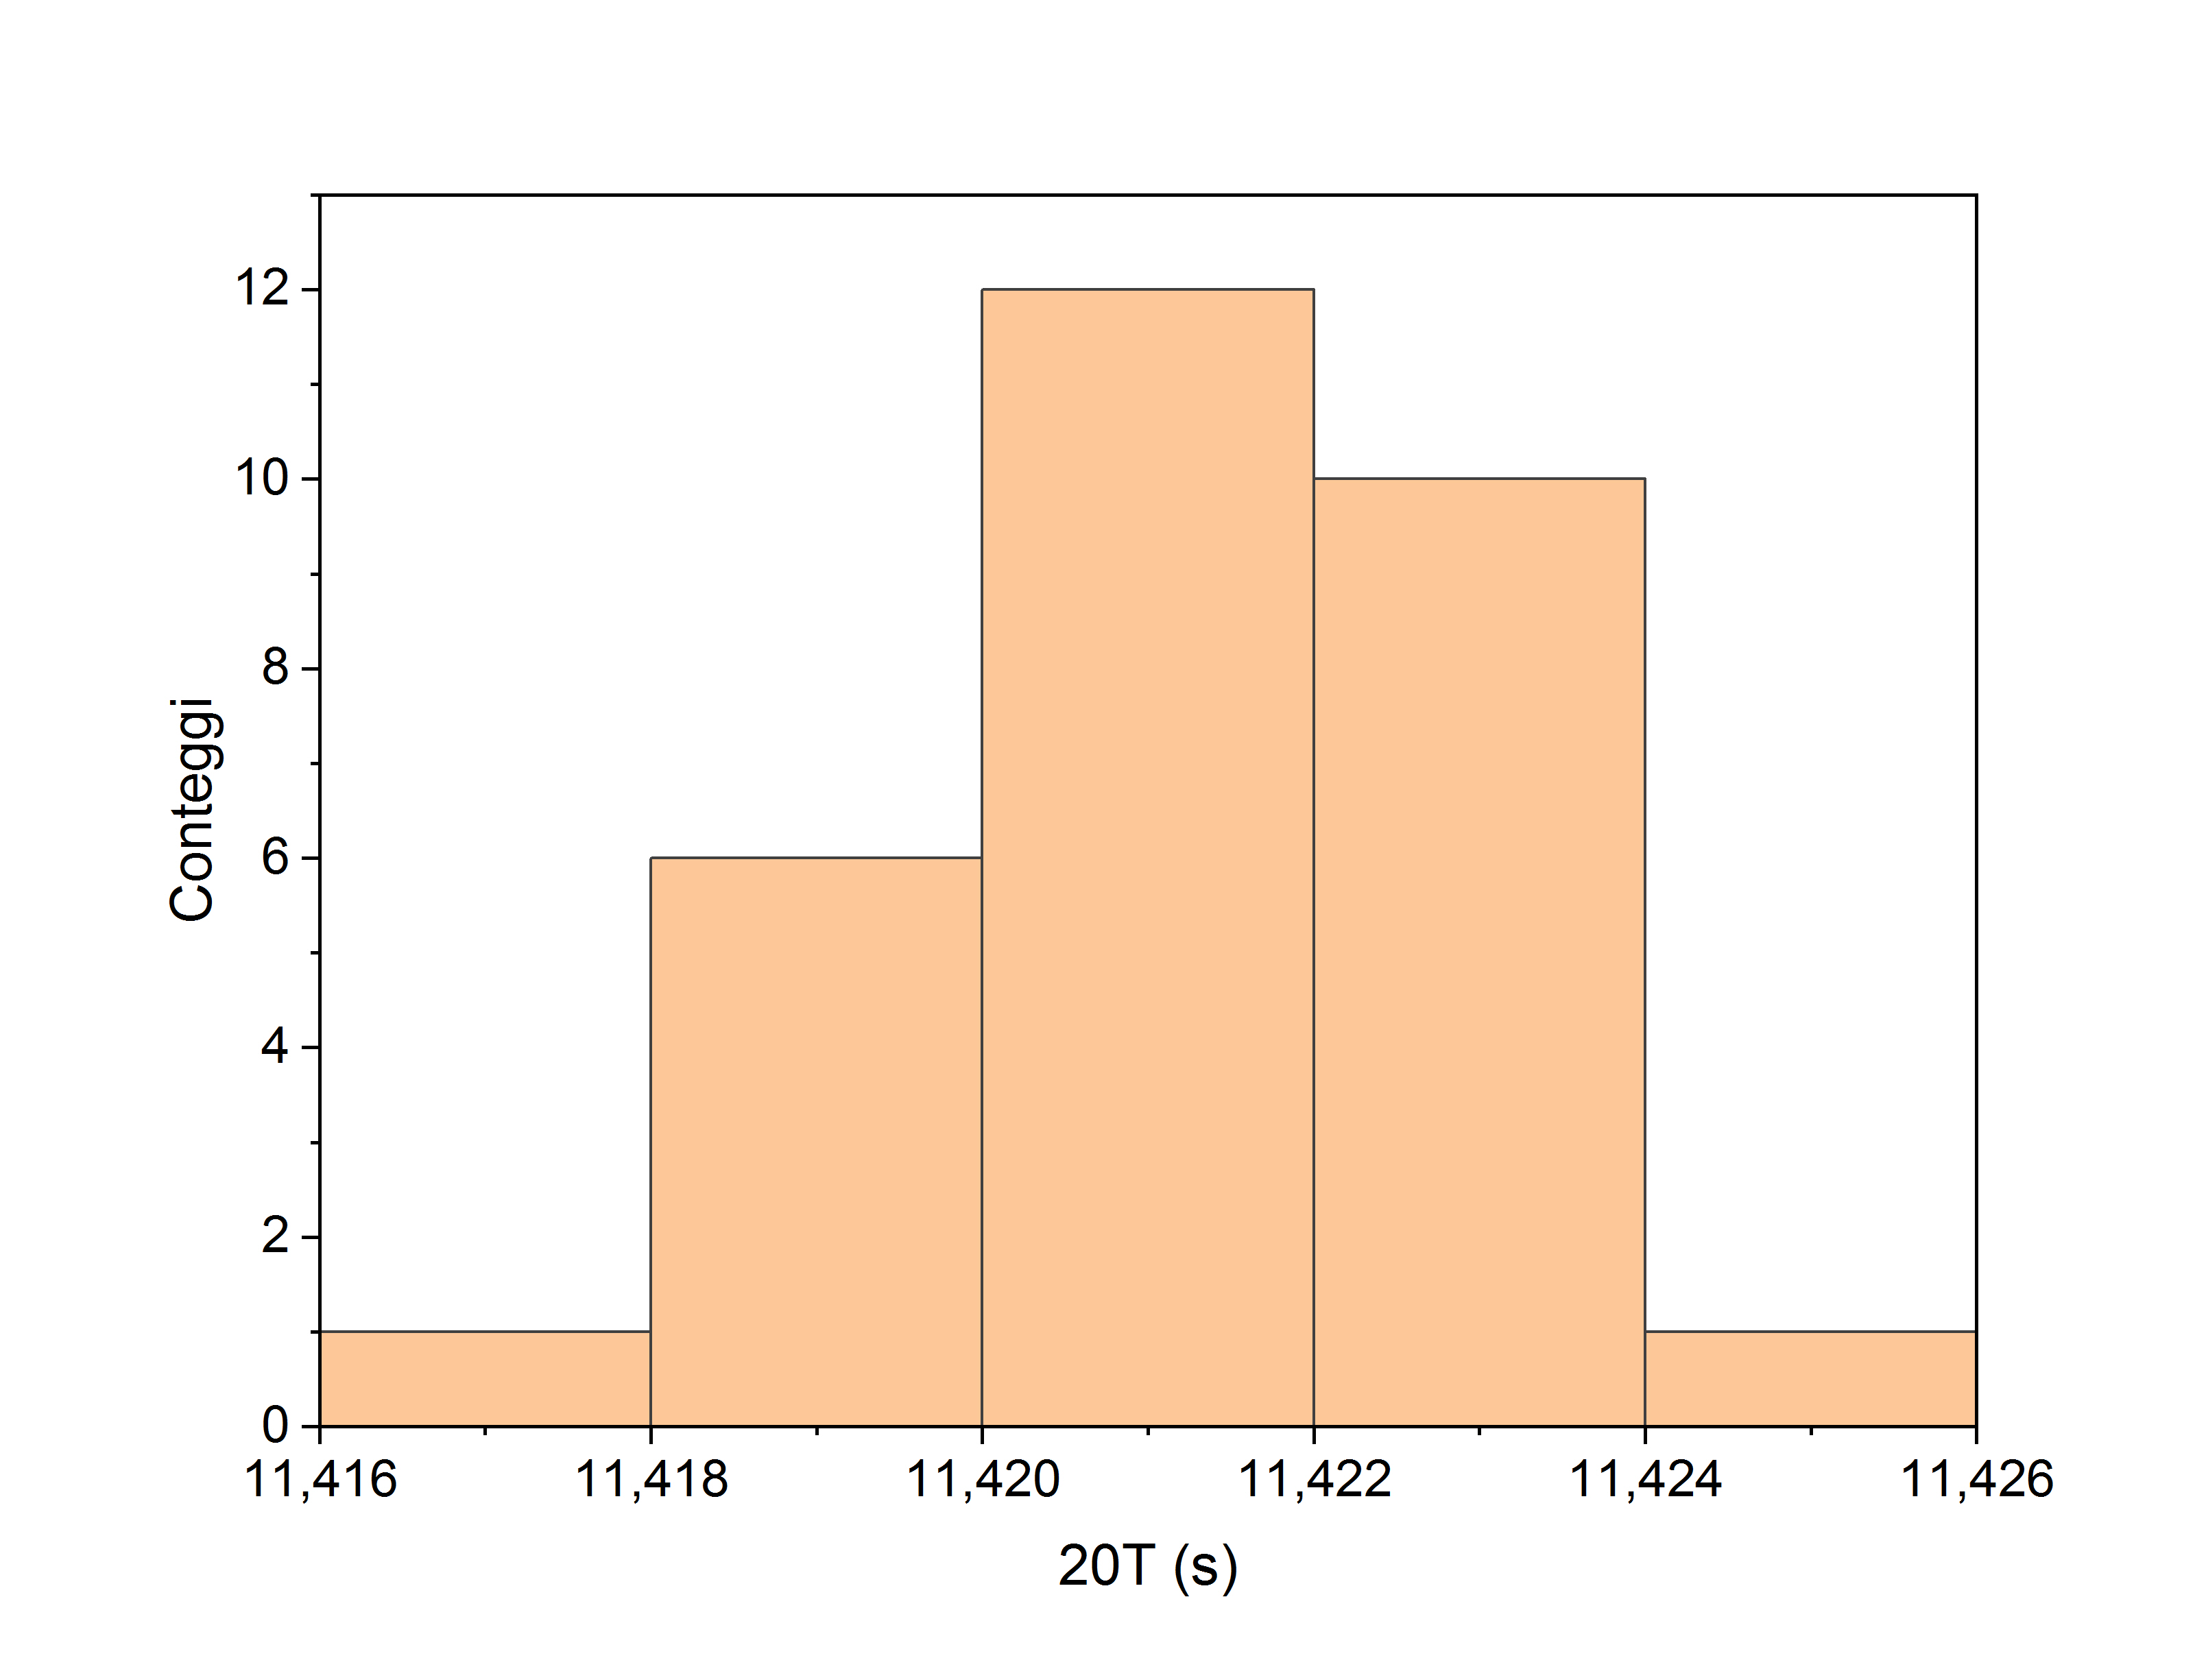
\includegraphics[trim={2cm 1.8cm .7cm 1.5cm},width=.5\textwidth]{Dinamico3.jpg}
    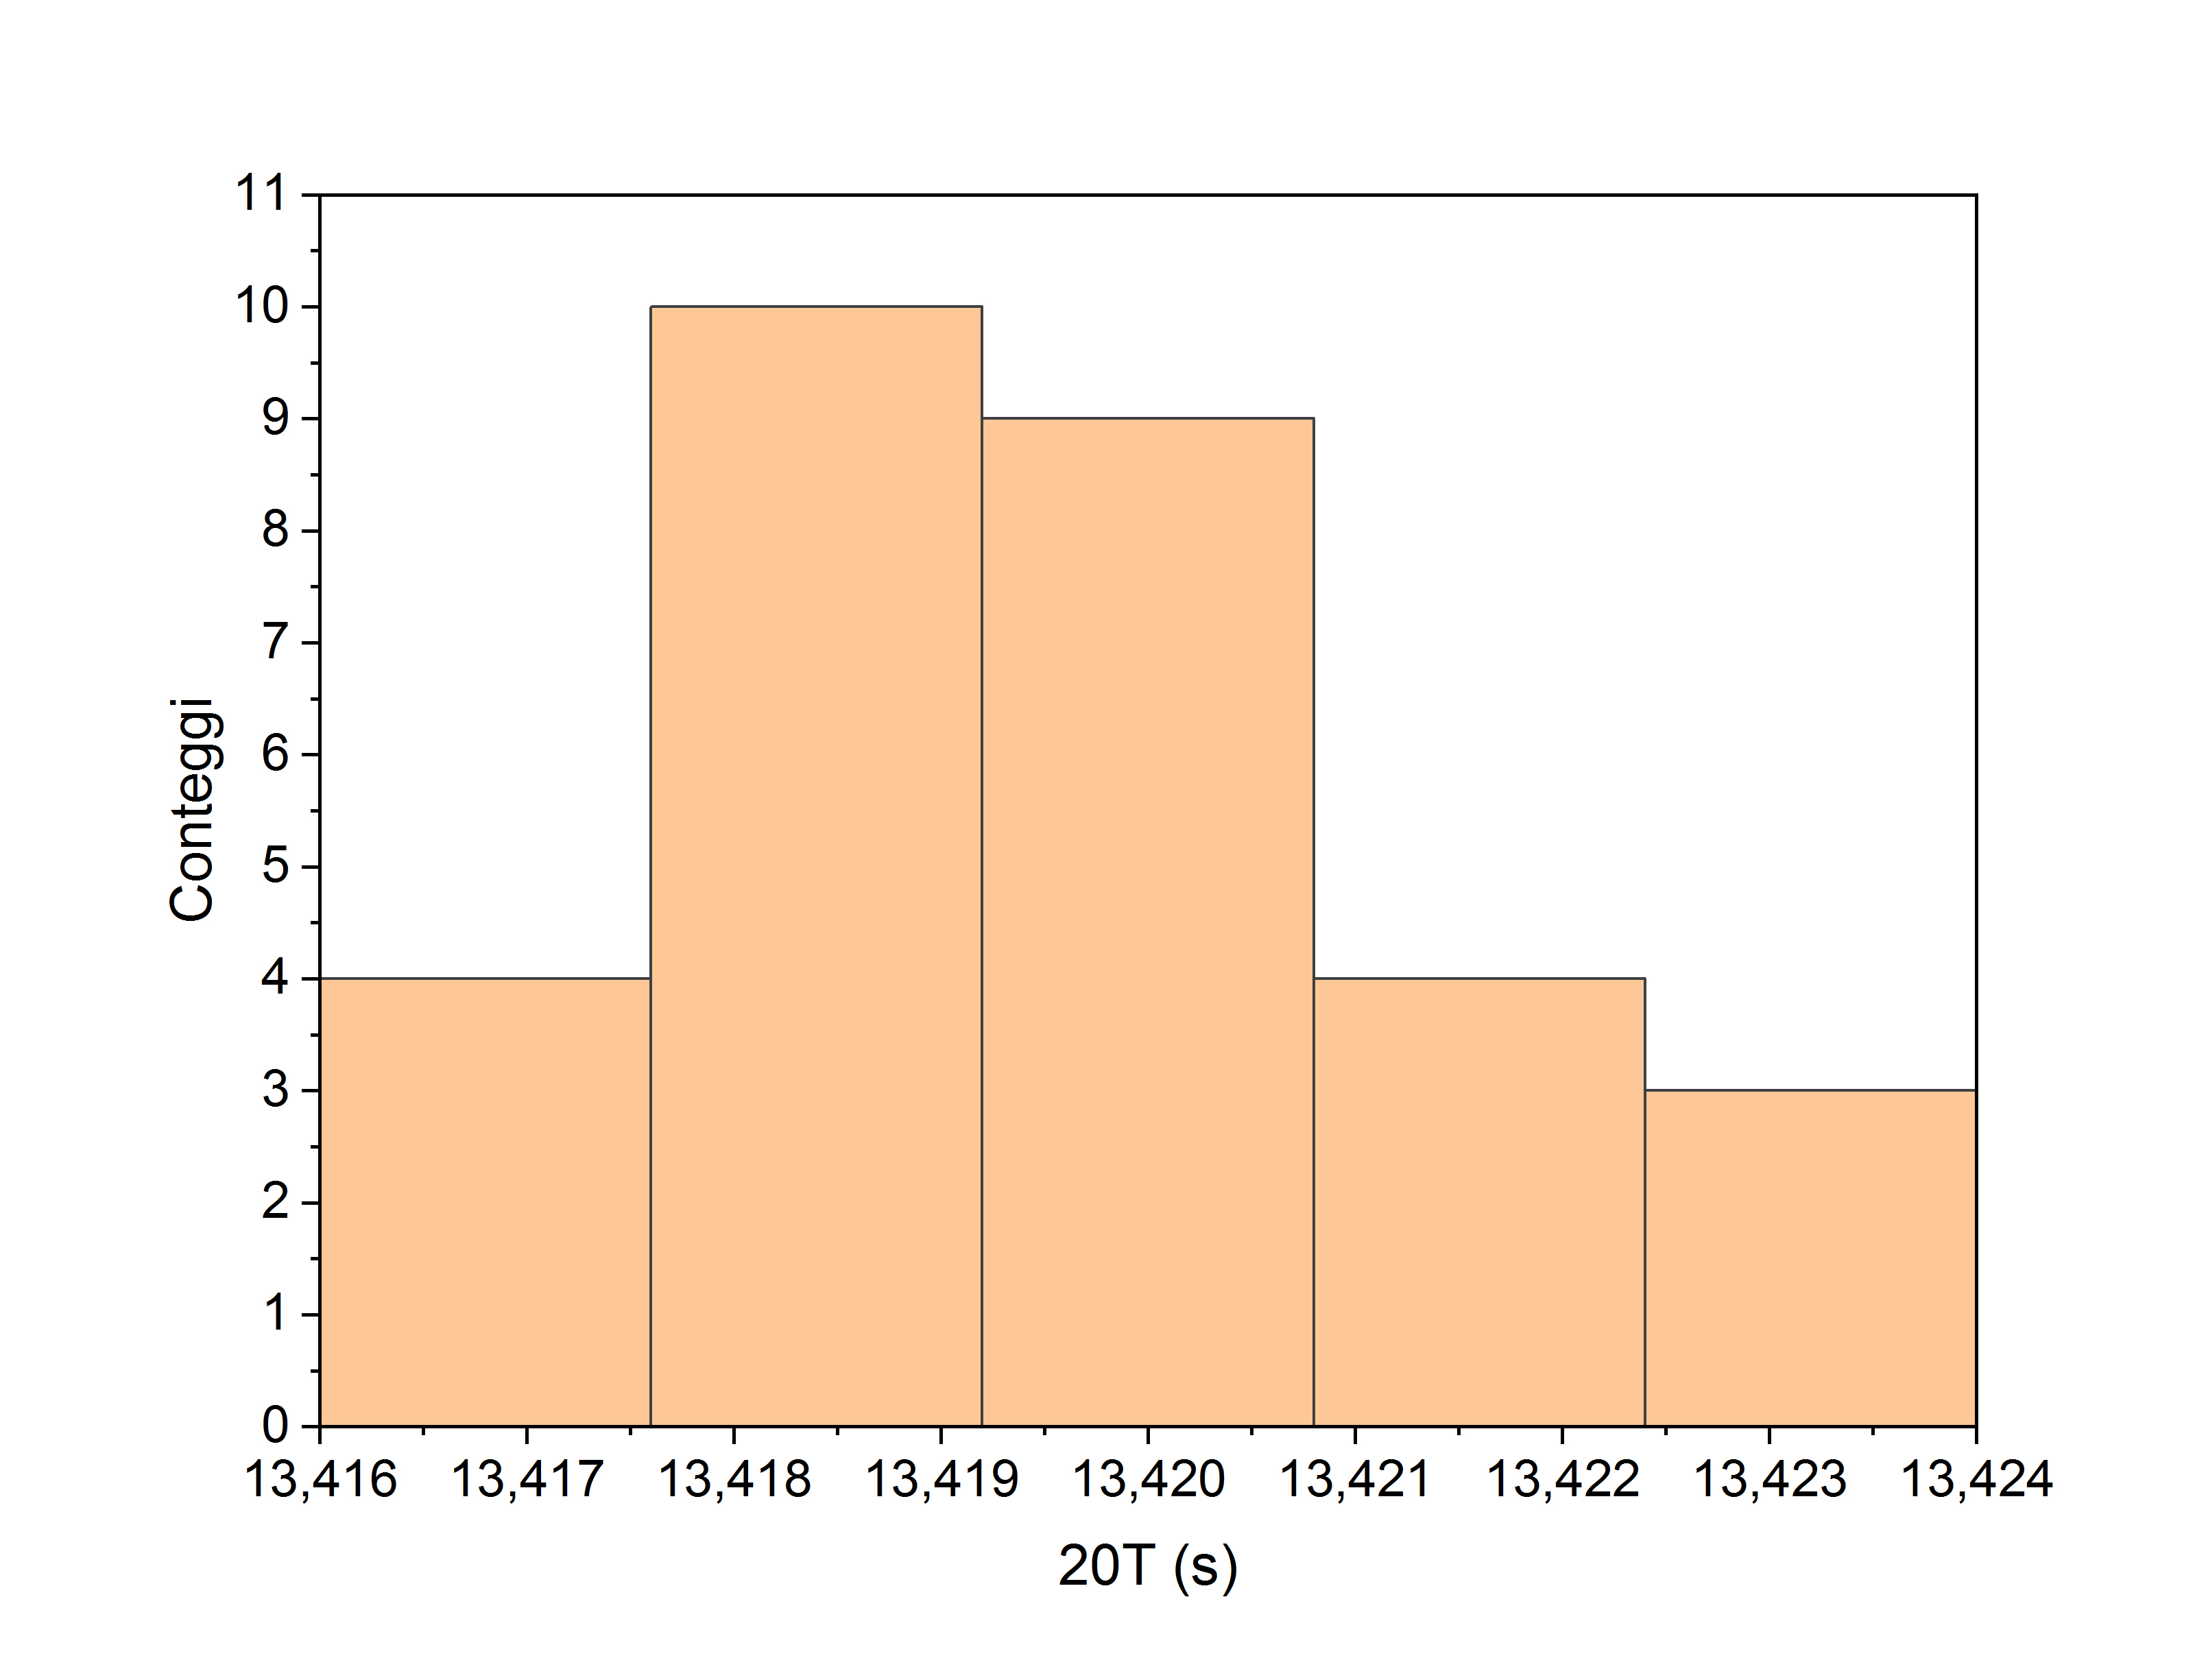
\includegraphics[trim={.7cm 1.8cm 2cm 1.5cm},width=.5\textwidth]{Dinamico4.jpg}
    \caption{Istogramma dei periodi delle oscillazioni di $C$ e $A+B$}
\end{figure}

Some more text

\begin{figure}[ht]
    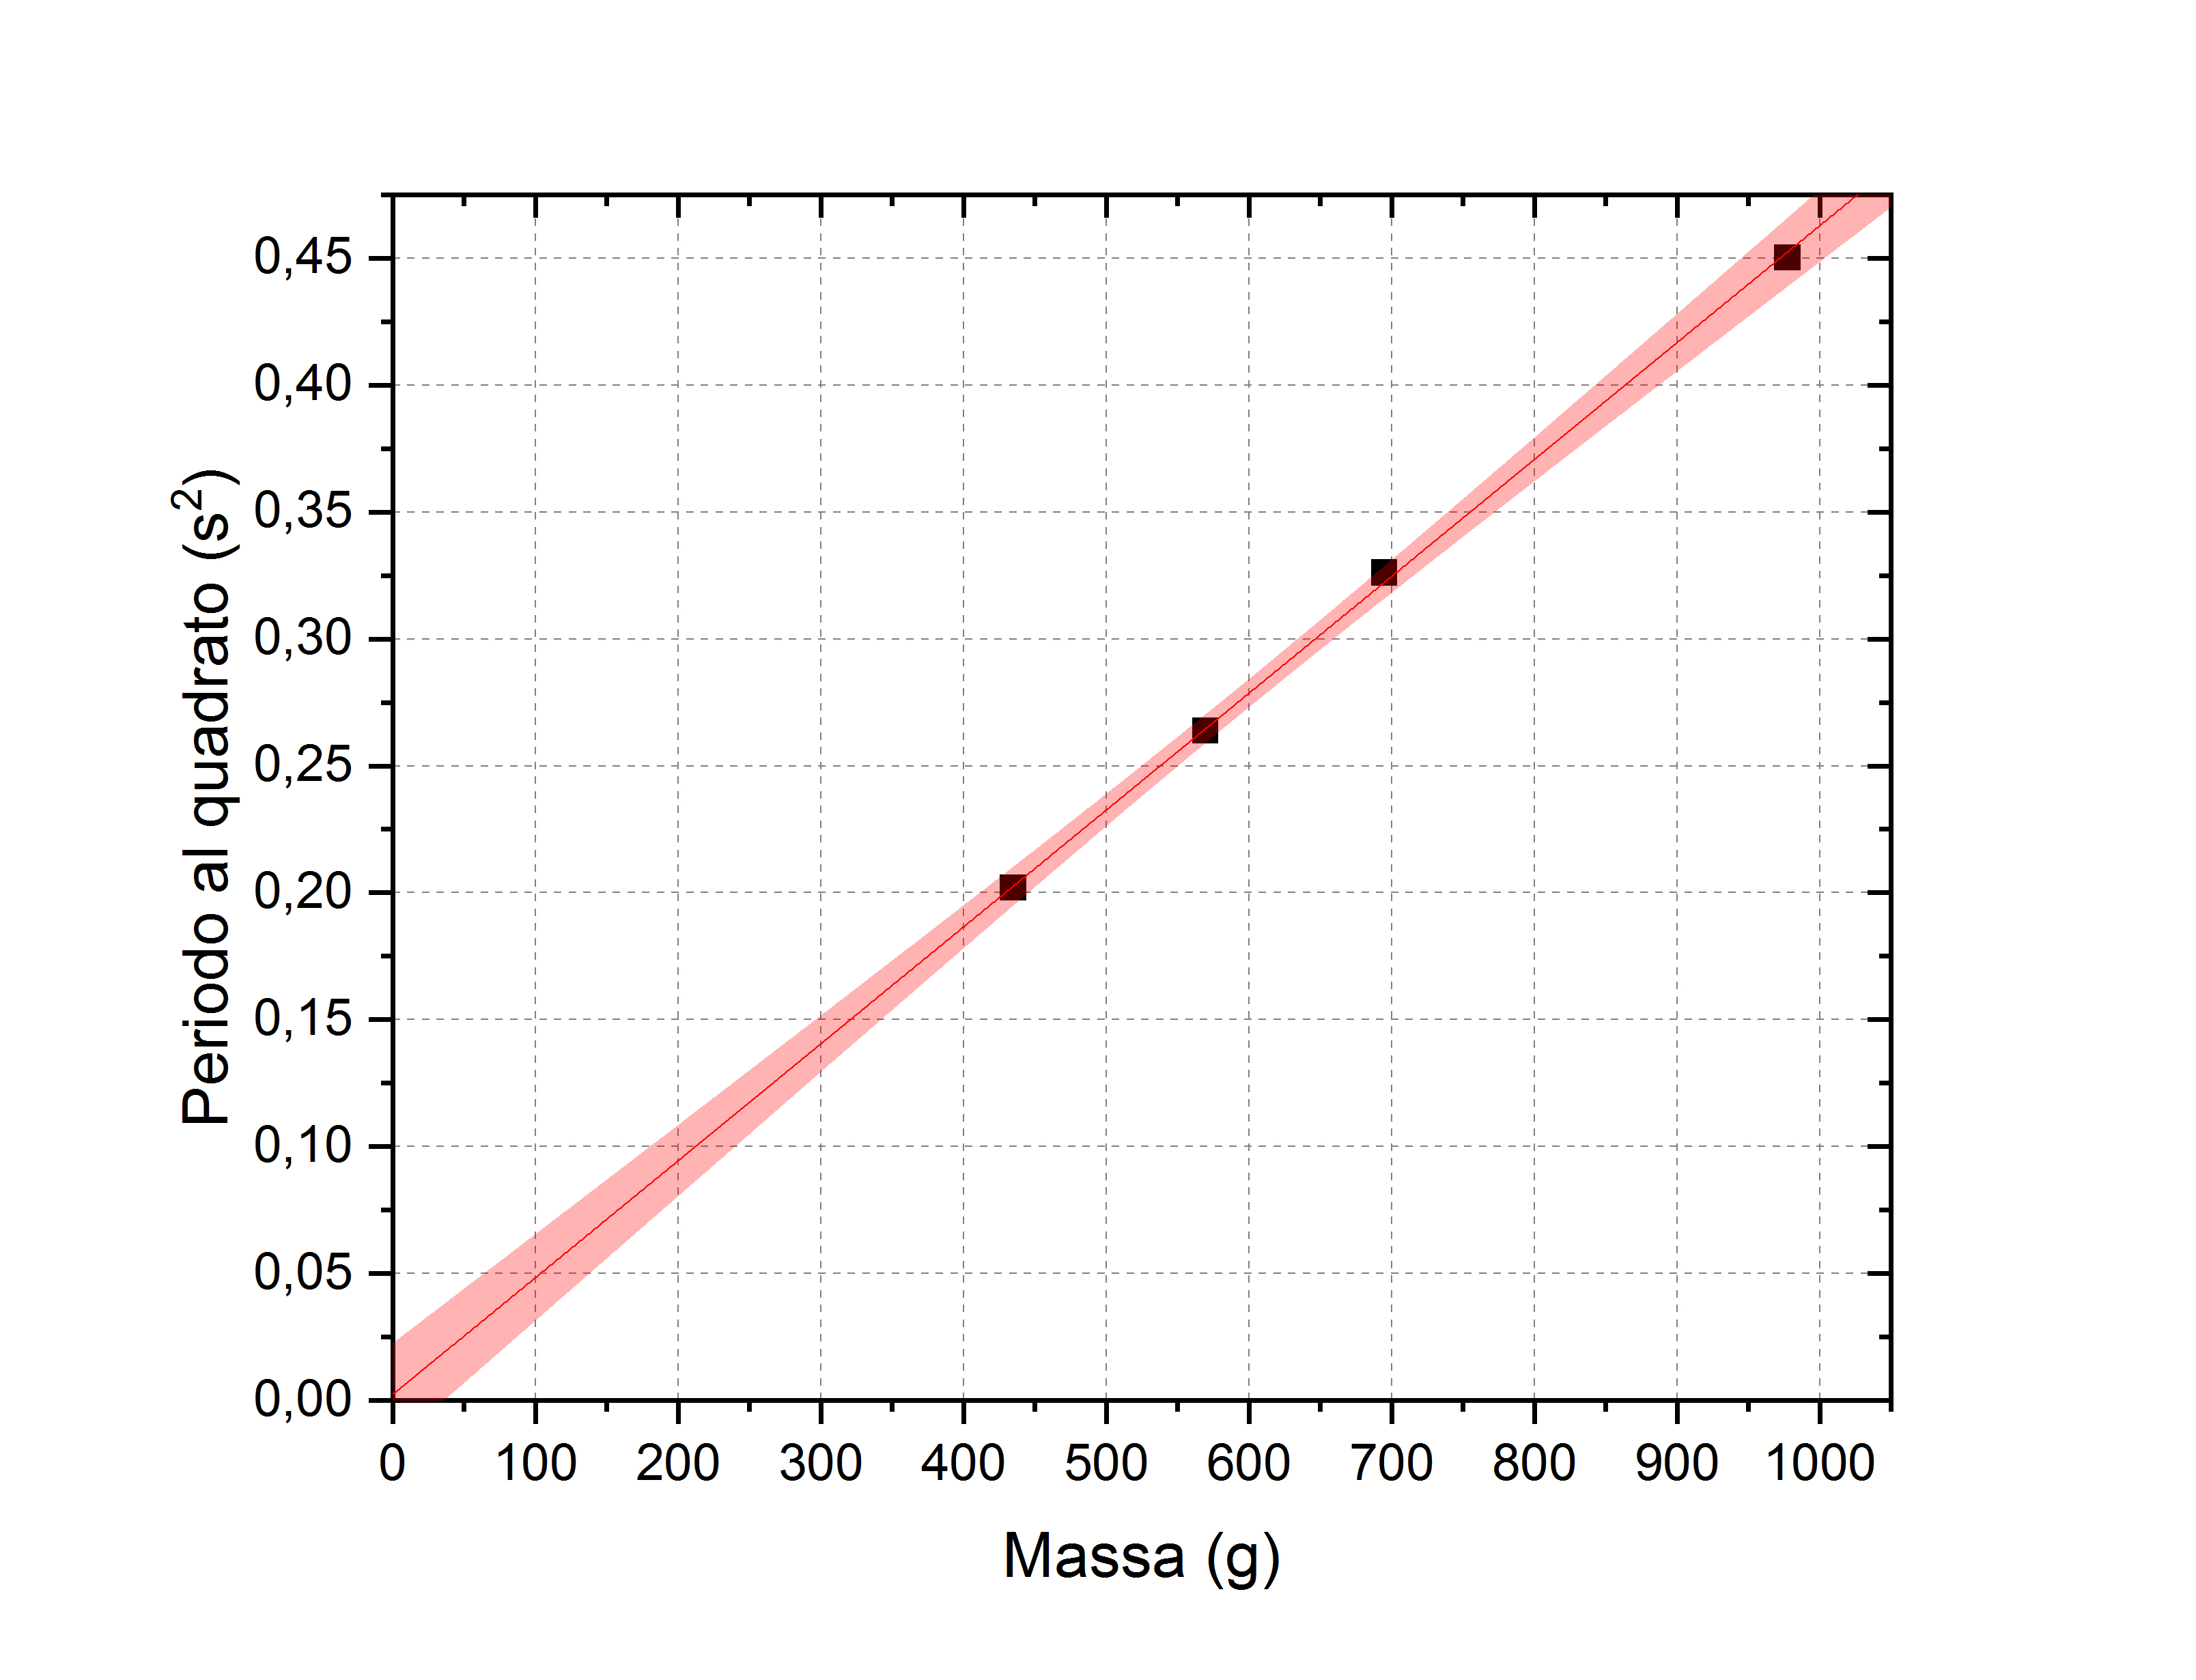
\includegraphics[trim={0 1.8cm 0 2cm},width=\textwidth]{DinamicoReg.jpg}
    \caption{Retta di regressione (in rosso) e la sua regione di incertezza (in rosa).}
\end{figure}

$a = ???$
$b = $

\section{Conclusioni}

L'inconsistenza non trascurabile tra $\rho$ (le nostre misure) e $\rho_\text{lett.}$ è dovuta principalmente al fatto che si tratta di leghe; probabilmente, i nostri campioni presentavano concentrazioni diverse dei vari elementi.


\footnotetext[1]{Text}

\end{document}
